\documentclass{standalone}
\usepackage{tikz}
\usetikzlibrary{patterns, positioning}


\begin{document}
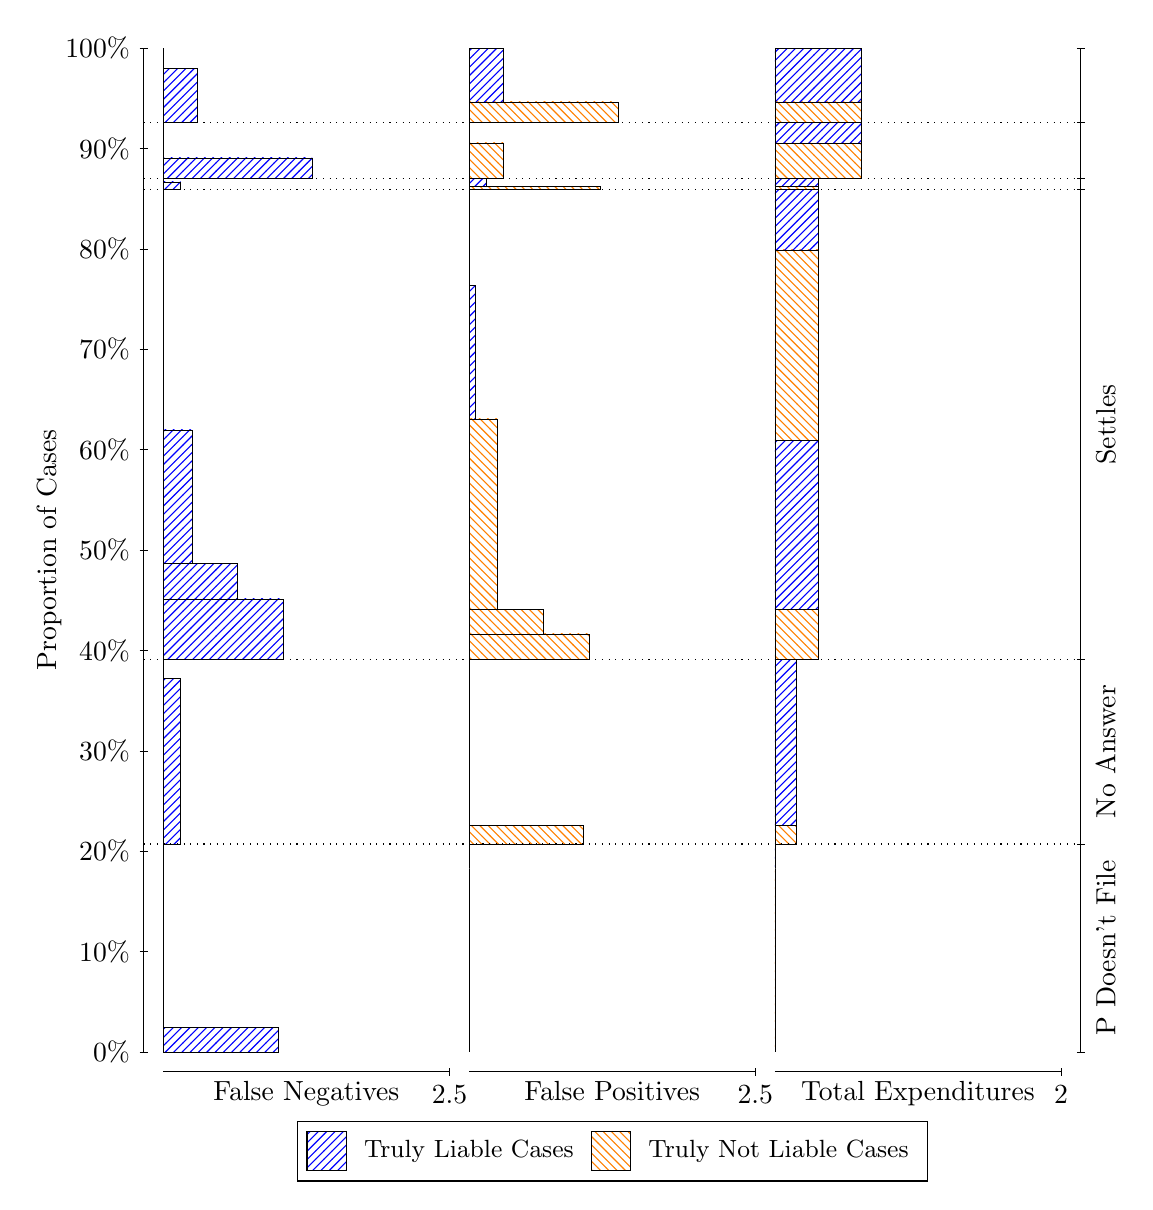
\begin{tikzpicture}
\draw[black, very thin] (1.5,1.75) -- (1.5,14.5);
\node[rotate=90, text=black, anchor=center] at (0.3, 8.125) {Proportion of Cases};
\draw[black, very thin] (1.45,1.75) -- (1.55,1.75);
\node[text=black, anchor=east] at (1.45, 1.75) {0\%};
\draw[black, very thin] (1.45,3.025) -- (1.55,3.025);
\node[text=black, anchor=east] at (1.45, 3.025) {10\%};
\draw[black, very thin] (1.45,4.3) -- (1.55,4.3);
\node[text=black, anchor=east] at (1.45, 4.3) {20\%};
\draw[black, very thin] (1.45,5.575) -- (1.55,5.575);
\node[text=black, anchor=east] at (1.45, 5.575) {30\%};
\draw[black, very thin] (1.45,6.85) -- (1.55,6.85);
\node[text=black, anchor=east] at (1.45, 6.85) {40\%};
\draw[black, very thin] (1.45,8.125) -- (1.55,8.125);
\node[text=black, anchor=east] at (1.45, 8.125) {50\%};
\draw[black, very thin] (1.45,9.4) -- (1.55,9.4);
\node[text=black, anchor=east] at (1.45, 9.4) {60\%};
\draw[black, very thin] (1.45,10.675) -- (1.55,10.675);
\node[text=black, anchor=east] at (1.45, 10.675) {70\%};
\draw[black, very thin] (1.45,11.95) -- (1.55,11.95);
\node[text=black, anchor=east] at (1.45, 11.95) {80\%};
\draw[black, very thin] (1.45,13.225) -- (1.55,13.225);
\node[text=black, anchor=east] at (1.45, 13.225) {90\%};
\draw[black, very thin] (1.45,14.5) -- (1.55,14.5);
\node[text=black, anchor=east] at (1.45, 14.5) {100\%};

\draw[black, very thin] (13.4,1.75) -- (13.4,14.5);
\draw[black, very thin] (13.35,1.75) -- (13.45,1.75);
\node[anchor=west] at (13.35, 1.75) {};
\draw[black, very thin] (13.35,4.3907) -- (13.45,4.3907);
\node[anchor=west] at (13.35, 4.3907) {};
\draw[black, very thin] (13.35,6.7366) -- (13.45,6.7366);
\node[anchor=west] at (13.35, 6.7366) {};
\draw[black, very thin] (13.35,12.704) -- (13.45,12.704);
\node[anchor=west] at (13.35, 12.704) {};
\draw[black, very thin] (13.35,12.843) -- (13.45,12.843);
\node[anchor=west] at (13.35, 12.843) {};
\draw[black, very thin] (13.35,13.556) -- (13.45,13.556);
\node[anchor=west] at (13.35, 13.556) {};
\draw[black, very thin] (13.35,14.5) -- (13.45,14.5);
\node[anchor=west] at (13.35, 14.5) {};

\draw[black, very thin, pattern color=blue, pattern=north east lines] (1.75,1.75) rectangle (3.2033,2.0615);
\draw[black, very thin, pattern color=orange, pattern=north west lines] (1.75,2.0615) rectangle (1.75,4.3907);
\draw[black, very thin, pattern color=blue, pattern=north east lines] (1.75,4.3907) rectangle (1.968,6.4984);
\draw[black, very thin, pattern color=orange, pattern=north west lines] (1.75,6.4984) rectangle (1.75,6.7366);
\draw[black, very thin, pattern color=blue, pattern=north east lines] (1.75,6.7366) rectangle (3.276,7.5043);
\draw[black, very thin, pattern color=blue, pattern=north east lines] (1.75,7.5043) rectangle (2.6947,7.955);
\draw[black, very thin, pattern color=blue, pattern=north east lines] (1.75,7.955) rectangle (2.1133,9.6512);
\draw[black, very thin, pattern color=orange, pattern=north west lines] (1.75,9.6512) rectangle (1.75,12.704);
\draw[black, very thin, pattern color=blue, pattern=north east lines] (1.75,12.704) rectangle (1.968,12.801);
\draw[black, very thin, pattern color=orange, pattern=north west lines] (1.75,12.801) rectangle (1.75,12.843);
\draw[black, very thin, pattern color=blue, pattern=north east lines] (1.75,12.843) rectangle (3.6393,13.104);
\draw[black, very thin, pattern color=orange, pattern=north west lines] (1.75,13.104) rectangle (1.75,13.556);
\draw[black, very thin, pattern color=blue, pattern=north east lines] (1.75,13.556) rectangle (2.186,14.239);
\draw[black, very thin, pattern color=orange, pattern=north west lines] (1.75,14.239) rectangle (1.75,14.5);
\draw[black, very thin, pattern color=orange, pattern=north west lines] (5.6333,1.75) rectangle (5.6333,4.0792);
\draw[black, very thin, pattern color=blue, pattern=north east lines] (5.6333,4.0792) rectangle (5.6333,4.3907);
\draw[black, very thin, pattern color=orange, pattern=north west lines] (5.6333,4.3907) rectangle (7.0867,4.6289);
\draw[black, very thin, pattern color=blue, pattern=north east lines] (5.6333,4.6289) rectangle (5.6333,6.7366);
\draw[black, very thin, pattern color=orange, pattern=north west lines] (5.6333,6.7366) rectangle (7.1593,7.0584);
\draw[black, very thin, pattern color=orange, pattern=north west lines] (5.6333,7.0584) rectangle (6.578,7.3676);
\draw[black, very thin, pattern color=orange, pattern=north west lines] (5.6333,7.3676) rectangle (5.9967,9.7891);
\draw[black, very thin, pattern color=blue, pattern=north east lines] (5.6333,9.7891) rectangle (5.706,11.485);
\draw[black, very thin, pattern color=blue, pattern=north east lines] (5.6333,11.485) rectangle (5.6333,12.704);
\draw[black, very thin, pattern color=orange, pattern=north west lines] (5.6333,12.704) rectangle (7.3047,12.746);
\draw[black, very thin, pattern color=blue, pattern=north east lines] (5.6333,12.746) rectangle (5.8513,12.843);
\draw[black, very thin, pattern color=orange, pattern=north west lines] (5.6333,12.843) rectangle (6.0693,13.296);
\draw[black, very thin, pattern color=blue, pattern=north east lines] (5.6333,13.296) rectangle (5.6333,13.556);
\draw[black, very thin, pattern color=orange, pattern=north west lines] (5.6333,13.556) rectangle (7.5227,13.817);
\draw[black, very thin, pattern color=blue, pattern=north east lines] (5.6333,13.817) rectangle (6.0693,14.5);
\draw[black, very thin, pattern color=orange, pattern=north west lines] (9.5167,1.75) rectangle (9.5167,4.0792);
\draw[black, very thin, pattern color=blue, pattern=north east lines] (9.5167,4.0792) rectangle (9.5167,4.3907);
\draw[black, very thin, pattern color=orange, pattern=north west lines] (9.5167,4.3907) rectangle (9.7892,4.6289);
\draw[black, very thin, pattern color=blue, pattern=north east lines] (9.5167,4.6289) rectangle (9.7892,6.7366);
\draw[black, very thin, pattern color=orange, pattern=north west lines] (9.5167,6.7366) rectangle (10.062,7.3676);
\draw[black, very thin, pattern color=blue, pattern=north east lines] (9.5167,7.3676) rectangle (10.062,9.5144);
\draw[black, very thin, pattern color=orange, pattern=north west lines] (9.5167,9.5144) rectangle (10.062,11.936);
\draw[black, very thin, pattern color=blue, pattern=north east lines] (9.5167,11.936) rectangle (10.062,12.704);
\draw[black, very thin, pattern color=orange, pattern=north west lines] (9.5167,12.704) rectangle (10.062,12.746);
\draw[black, very thin, pattern color=blue, pattern=north east lines] (9.5167,12.746) rectangle (10.062,12.843);
\draw[black, very thin, pattern color=orange, pattern=north west lines] (9.5167,12.843) rectangle (10.607,13.296);
\draw[black, very thin, pattern color=blue, pattern=north east lines] (9.5167,13.296) rectangle (10.607,13.556);
\draw[black, very thin, pattern color=orange, pattern=north west lines] (9.5167,13.556) rectangle (10.607,13.817);
\draw[black, very thin, pattern color=blue, pattern=north east lines] (9.5167,13.817) rectangle (10.607,14.5);
\draw[black, dotted] (1.5,4.3907) -- (13.4,4.3907);
\draw[black, dotted] (1.5,6.7366) -- (13.4,6.7366);
\draw[black, dotted] (1.5,12.704) -- (13.4,12.704);
\draw[black, dotted] (1.5,12.843) -- (13.4,12.843);
\draw[black, dotted] (1.5,13.556) -- (13.4,13.556);
\draw[black, very thin] (1.75,1.5) -- (5.3833,1.5);
\node[text=black, anchor=north] at (3.5667, 1.5) {False Negatives};
\draw[black, very thin] (5.3833,1.45) -- (5.3833,1.55);
\node[text=black, anchor=north] at (5.3833, 1.45) {2.5};

\draw[black, very thin] (5.6333,1.5) -- (9.2667,1.5);
\node[text=black, anchor=north] at (7.45, 1.5) {False Positives};
\draw[black, very thin] (9.2667,1.45) -- (9.2667,1.55);
\node[text=black, anchor=north] at (9.2667, 1.45) {2.5};

\draw[black, very thin] (9.5167,1.5) -- (13.15,1.5);
\node[text=black, anchor=north] at (11.333, 1.5) {Total Expenditures};
\draw[black, very thin] (13.15,1.45) -- (13.15,1.55);
\node[text=black, anchor=north] at (13.15, 1.45) {2};

\node[text=black, centered, rotate=90] at (13.72, 3.0704) {P Doesn't File};
\node[text=black, centered, rotate=90] at (13.72, 5.5637) {No Answer};
\node[text=black, centered, rotate=90] at (13.72, 9.7201) {Settles};




\draw (7.449999999999999,1.5) node[draw=none] (baseCoordinate) {};
\begin{scope}[align=center]
        \matrix[scale=0.5, draw=black, below=0.5cm of baseCoordinate, nodes={draw}, column sep=0.1cm]{
            \node[rectangle, draw, minimum width=0.5cm, minimum height=0.5cm, pattern color=blue, pattern=north east lines] {}; &
            \node[draw=none, font=\small, text=black] (B) {Truly Liable Cases}; &
            \node[rectangle, draw, minimum width=0.5cm, minimum height=0.5cm, pattern color=orange, pattern=north west lines] {}; &
            \node[draw=none, font=\small, text=black] (B) {Truly Not Liable Cases}; \\
            };
\end{scope}

\end{tikzpicture}
\end{document}